\section{Programação dinâmica em uma árvore fixa}
\label{sec:fixed-dp}

Seja $T$ uma árvore diádica fixa, enraizada em $K$, e de profundidade
relativa no máximo $D$. Para um nó $J$ de $T$ e
$u,v\in\Values_{D,H}(K)$, denote por
\[
 \Representations_H(T_J;u,v)
\]
o conjunto das rotulações contínuas da subárvore $T_J$ por átomos de
$\Library_H$ que assumem $u$ e $v$ nas extremidades de $J$. O conjunto pode
ser vazio.

\begin{definition}[recorrência para árvore fixa]
\label{def:fixed-recurrence}
Defina $C_T(J;u,v)$ de baixo para cima. Se $J$ é folha de $T$,
\begin{equation}
 C_T(J;u,v)=\Phi_H(J;u,v).
 \label{eq:fixed-leaf}
\end{equation}
Se $J$ é interno, com filhos $J_L,J_R$, defina
\begin{equation}
 C_T(J;u,v)=\lambda_{\rm bits}+\lambda_{\rm split}
 +\min_{w\in\Values_{D,H}(K)}
 \{C_T(J_L;u,w)+C_T(J_R;w,v)\}.
 \label{eq:fixed-split}
\end{equation}
Adota-se $\min\varnothing=+\infty$ e as regras usuais para soma com
$+\infty$.
\end{definition}

O valor intermediário $w$ aparece simultaneamente como extremo direito da
subárvore esquerda e extremo esquerdo da subárvore direita. Ele é exatamente
o acoplamento de continuidade que se perderia em um estado contendo apenas a
célula; a \cref{fig:boundary-state} mostra essa junção.

\begin{figure}[t]
 \centering
 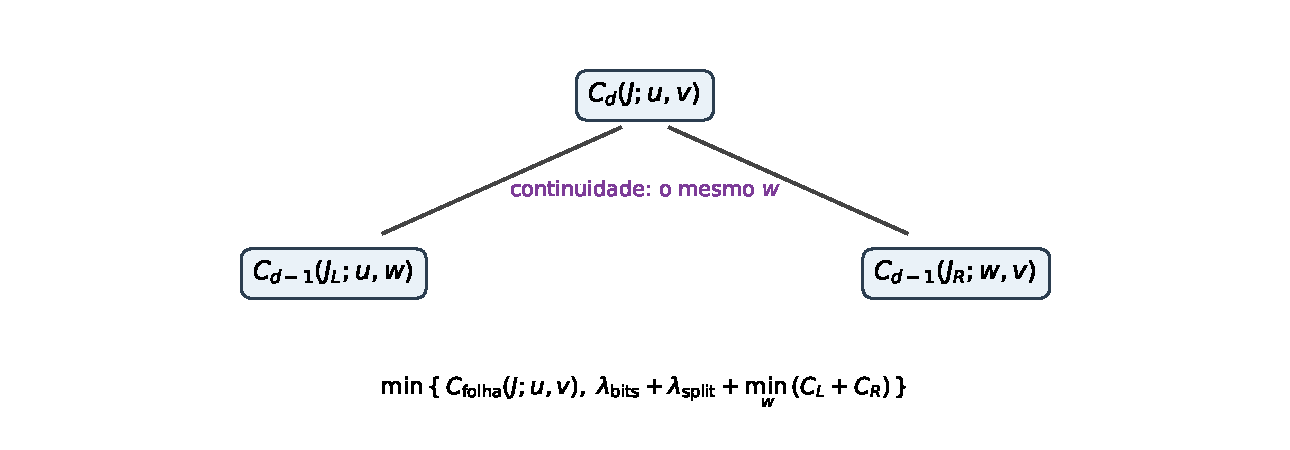
\includegraphics[width=.92\linewidth]{fig01_estado_fronteira.pdf}
 \caption{O estado registra os dois valores externos; o valor $w$ é
 compartilhado pelos filhos e impõe continuidade. O termo de subdivisão
 inclui o bit do nó interno e a penalidade estrutural.}
 \label{fig:boundary-state}
\end{figure}

\begin{theorem}[correção para árvore fixa]
\label{thm:fixed-correctness}
Para todo nó $J$ de $T$ e todo par de estados $(u,v)$,
\begin{equation}
 C_T(J;u,v)
 =\min_{R\in\Representations_H(T_J;u,v)}
 \cost_{\mathcal Z}(R),
 \label{eq:fixed-correctness}
\end{equation}
com valor $+\infty$ se o conjunto à direita for vazio. Se, em cada mínimo,
for armazenado também o candidato de menor chave \eqref{eq:tie-key}, a
retropropagação reconstrói uma única representação canônica. Em particular,
\begin{equation}
 \min_{u,v\in\Values_{D,H}(K)}C_T(K;u,v)
 =\min_{R\in\Representations_H(T)}\cost_{\mathcal Z}(R).
 \label{eq:fixed-global}
\end{equation}
\end{theorem}

\begin{proof}
Proceda por indução na altura da subárvore. Se $J$ é folha, a
\cref{prop:endpoint-dictionary} mostra que existe exatamente um rótulo com
fronteiras $(u,v)$ quando $(u,v)\in\Pairs_H(J)$, e nenhum nos demais casos.
Seu custo é precisamente \eqref{eq:leaf-cost}, provando
\eqref{eq:fixed-leaf}.

Suponha agora que $J$ tenha filhos. Toda montagem contínua em $T_J$ possui um
único valor $w$ na fronteira compartilhada. Sua restrição aos filhos pertence
a
\[
 \Representations_H(T_{J_L};u,w)
 \quad\text{e}\quad
 \Representations_H(T_{J_R};w,v).
\]
Reciprocamente, quaisquer duas representações desses conjuntos colam-se em
uma representação contínua de $T_J$. Pelo \cref{lem:recursive-stream}, a
colagem acrescenta um bit de nó interno; ela também acrescenta uma
subdivisão. A aditividade da perda e das duas penalidades dá
\eqref{eq:fixed-split}. Aplicar a hipótese de indução aos dois filhos prova
\eqref{eq:fixed-correctness}.

Há um número finito de estados e candidatos. A ordem de
\eqref{eq:tie-key} é total e, pelo \cref{lem:tie-concatenation}, guardar o
menor candidato em cada estado não elimina o minimizador canônico de nenhuma
superárvore. Os apontadores dos valores $w$ e das decisões recuperam esse
candidato. Minimizar também sobre os dois valores externos da raiz prova
\eqref{eq:fixed-global}.
\end{proof}

\begin{algorithm}[rotulação exata de uma árvore fixa]
\label{alg:fixed-tree}
Enumere $\Pairs_H(J)$ em cada folha. Percorra $T$ em pós-ordem. Em cada nó
interno, agrupe os estados do filho direito pelo valor de fronteira esquerdo
$w$ e una apenas pares com o mesmo $w$. Para cada estado externo $(u,v)$,
retenha a menor chave \eqref{eq:tie-key} e um apontador para os dois filhos.
Na raiz, escolha a menor entrada finita e siga os apontadores.
\end{algorithm}

O agrupamento por $w$ não altera a recorrência; ele apenas evita testar pares
de subárvores que violam continuidade de maneira evidente.
